\newpage
\section{Integracja sztucznej skóry z systemem robota}
\label{s_integracja}

\subsection{Środowisko pracy robota}

W testach został wykorzystany opisywany już w tej pracy robot Tiago, w konfiguracji bez dołączonych manipulatorów, lecz z uchwytem na tablet i czytnikiem NFC. Dodatkowo, do robota został dostawiony (położony na wierzchu robota) notebook z systemem Ubuntu 18.4 pozwalający w wygodny sposób obserwować i pracować na systemie ROS używanym przez robota. Został także dodany mikrofon dookolny o dużo lepszej jakości rejestrowanego dźwięku, niż ten wbudowany w robota. Mikrofon ten został podłączony bezpośrednio do notebooka. Został on także wykorzystany w innym projekcie w sterowaniu robotem za pomocą komend głosowych. Robot jest także podłączony do sieci WiFi i~przygotowany do pracy w~systemach IOT. Obecna konfiguracja robota, wraz z~dołączonymi peryferiami, została w~pełni przedstawiona na rysunku \ref{f_tiago_system} \cite{b_unpublic_system_lab}. 

\begin{figure}[!h]
    \centering 
    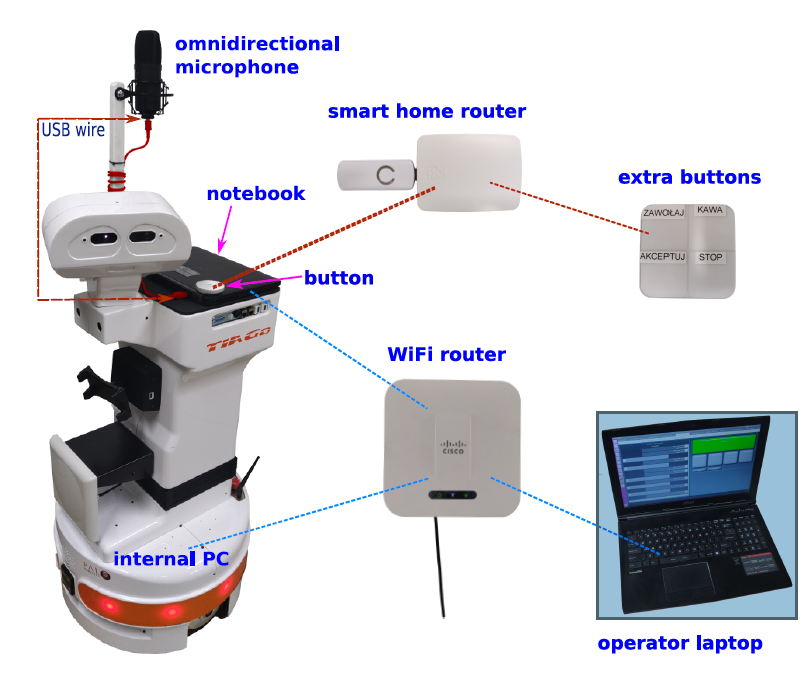
\includegraphics[width=0.9\linewidth]{img/tiago_system_lab.png}
    \caption{Robot Tiago wraz z dołączonym do niego systemem \cite{b_unpublic_system_lab}}
    \label{f_tiago_system}
\end{figure}

Tiago dostępny w laboratorium, podobnie jak jego symulacja, działa na systemie ROS w~wersji \textit{melodic}. W symulacji w dużej mierze wykorzystywane są pakiety dostarczane przez producenta - PAL Robotics, ale zostały obudowane przez dodatkowe pakiety zawierające m.in. mapę laboratorium robotycznego w~rzeczywistych wymiarach wraz z~odwzorowaniem przedmiotów znajdujących się w nim. Odwzorowane laboratorium w~programie Gazebo, wraz z~widocznym robotem, jest przedstawione na rysunku~\ref{f_lab_gazebo}. Widoczne na obrazku wyraźne niebieskie linie obrazują wiązki z~laserowego czujnika odległości i~skupiają się one przy robocie. 

\begin{figure}[!h]
    \centering 
    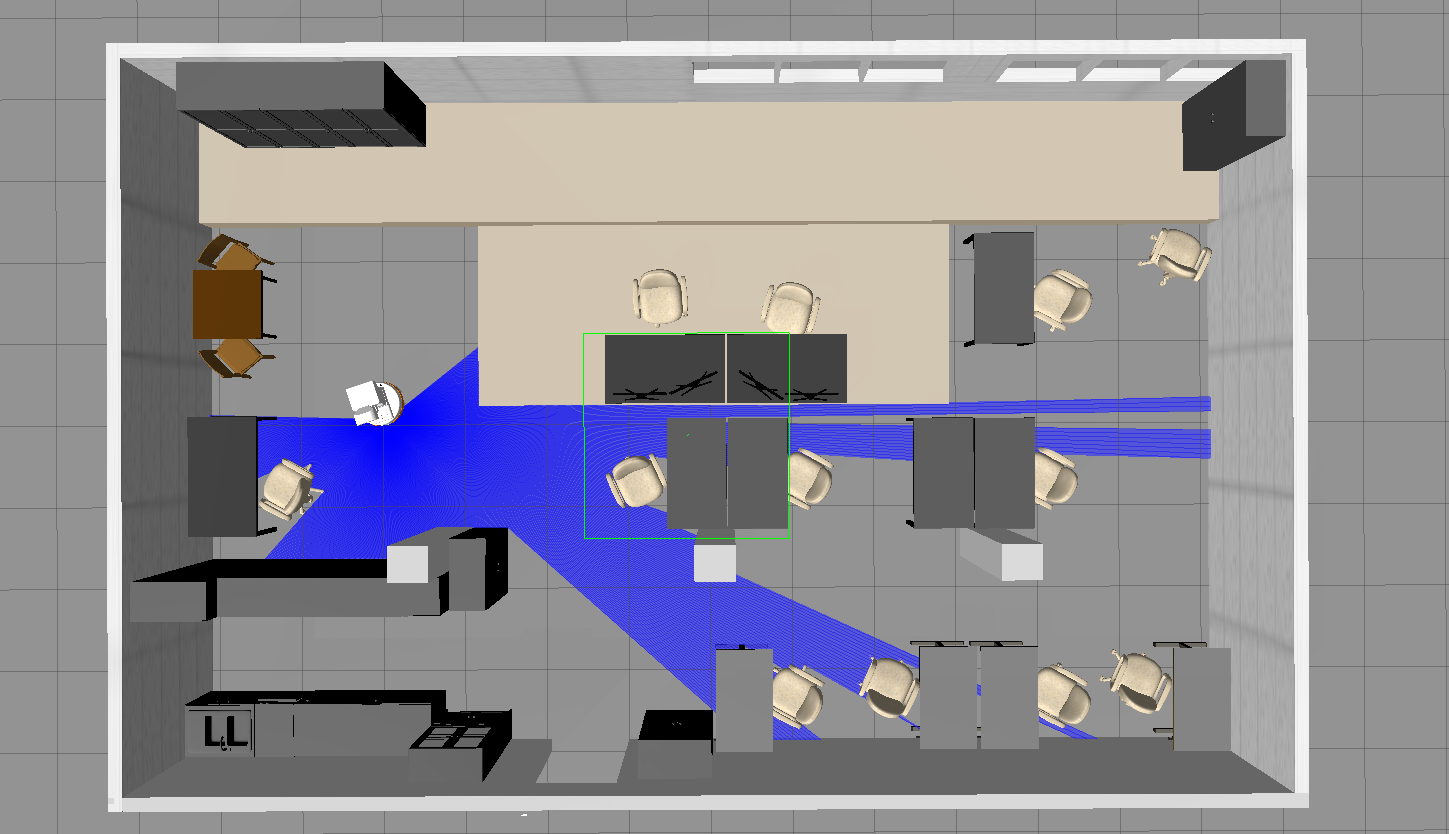
\includegraphics[width=0.95\linewidth]{img/ros_gazebo_lab.png}
    \caption{Laboratorium robotyczne odwzorowane w programie Gazebo}
    \label{f_lab_gazebo}
\end{figure}

\subsection{Budowa modułu sztucznej skóry mocowanego na robocie Tiago}
\label{ss_integracja_budowa}

Konstruowanie prototypu przeznaczonego do umieszczenia na robocie zostało zapoczątkowane przez dokładne zebranie wszystkich pomiarów z robota oraz zaplanowanie, jak projektowany czujnik będzie wyglądał. Zostało także wybrane dokładne umiejscowienie sztucznej skóry na robocie, jak również ustalono za ochronę których części będzie on odpowiadał. W ten sposób wywnioskowano, że czujnik powinien się znajdować w~górnej części robota. Tiago w~górnej części nie posiada żadnych czujników odległości i~jest bardziej narażony na przypadkowe uderzenia przez człowieka lub wiszące przedmioty. Czujnik planowo został zaprojektowany tylko do ochraniania tylnej i bocznych części robota. Przednia część nie była chroniona, ponieważ jest w niej umiejscowiona głowa, której ochrona wymaga użycia bardziej skomplikowanych kształtów czujnika. Użycie niewyprofilowanego czujnika wiązałoby się z sporym wyjściem poza istniejący obrys robota. Dodatkowo, zamontowany czujnik nie może w żaden sposób blokować ruchów głowy robota.

Szkielet sztucznej skóry zbudowany został z dociętej na wymiar płyty MDF o grubości $6 mm$. Jest to materiał lekki, o niewielkiej grubości, a jednocześnie wystarczająco sztywny, aby nie uginać się pod wpływem siły wywieranej na sztuczną skórę. Dodatkowymi plusami przemawiającymi za jego wyborem są duża dostępność, niska cena i bardzo łatwa obróbka.

% TODO zdjęcie szkieletu??

Do tak przygotowanego szkieletu przymocowana została za pomocą taśmy dwustronnej sztuczna skóra wykonana na wymiary szkieletu.
Kolejne warstwy sztucznej skóry zostały zbudowane z dobranej wcześniej gumy o grubości $10 mm$ przeznaczonej na warstwę wewnętrzną czujnika. Taśma dwustronna jest do jej zamocowania w pełni wystarczalna, z~powodu małej masy całego czujnika. Do warstwy wewnętrznej przymocowane zostały pionowe paski taśmy miedzianej o szerokości $25 mm$ z dolutowanymi w ich górnej części przewodami. Zastosowanie węższych pasków pozwala zwiększyć dokładność wykrywania kierunku, z którego wywierany jest nacisk. Do tak przygotowanej wewnętrznej warstwy doklejony został swobodnie zwisający kawałek folii Velostat. Swobodne ułożenie folii jest konieczne, ponieważ dowolne naprężenie folii zmniejsza jej rezystancję, co drastycznie wpływa na błędy w odczytywanych danych i~wprowadza duże zakłócenia. Do całości przymocowano również (taśmą dwustronną) zewnętrzny fragment gumy ochronnej o~grubości $5 mm$ z~przymocowanym do niego poziomym paskiem folii miedzianej o~szerokości $50 mm$. W tym przypadku pas folii miedzianej jest szerszy, ponieważ korzystając z~pojedynczego poziomego paska folii ważne jest, aby zbierał on  naciski z jak najszerszego obszaru. Zbudowany w~ten~sposób czujnik w opisywanej konfiguracji mocowanej na tył robota widoczny jest na zdjęciu \ref{f_szkielet_obity}.

\begin{figure}[!h]
  \begin{subfigure}[t]{0.5\linewidth}
    \centering
    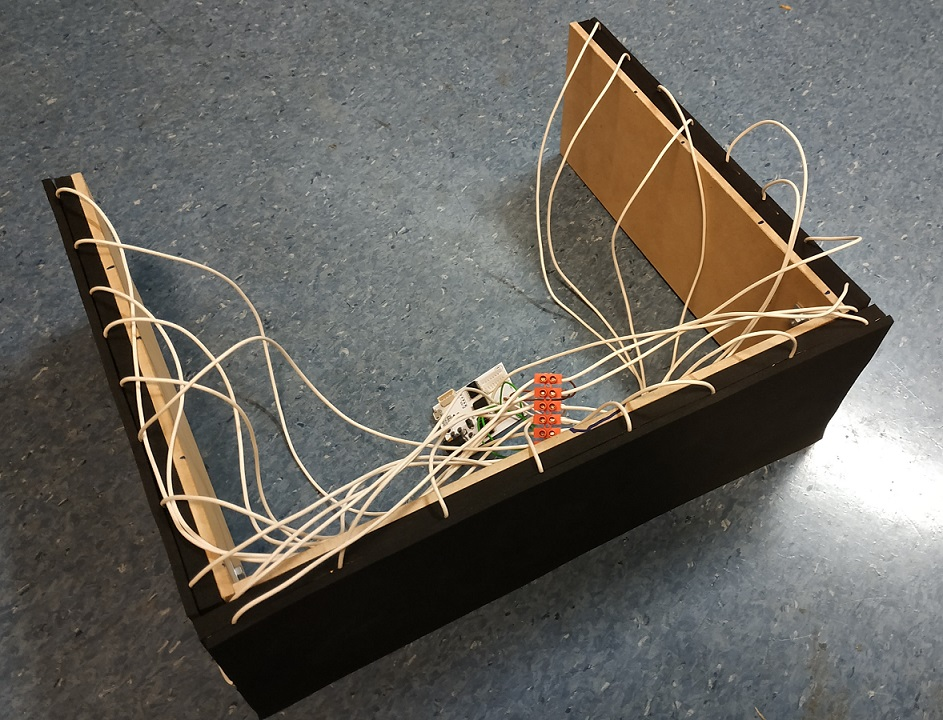
\includegraphics[width=0.85\linewidth]{img/szkielet_obity_przod.jpg} 
    \caption{Widok z zewnątrz prototypu} 
    % \vspace{4ex}
  \end{subfigure}%% 
  \begin{subfigure}[t]{0.487\linewidth}
    \centering
    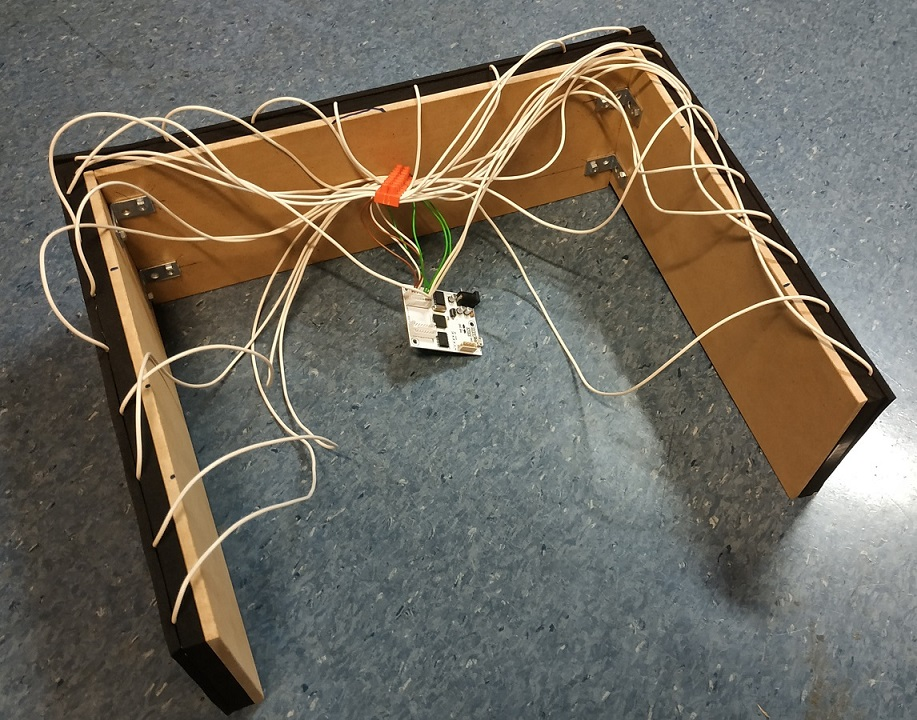
\includegraphics[width=0.85\linewidth]{img/szkielet_obity_tyl.jpg}
    \caption{Widok od wnętrza prototypu} 
    % \vspace{4ex}
  \end{subfigure}
  
  \centering
  \caption{Zbudowany prototyp przeznaczony do zamocowania na robocie}
  \label{f_szkielet_obity}
\end{figure}

Konfiguracja sztucznej skóry została wykonana analogicznie jak podczas testów opisywanych w sekcji \ref{sss_budowa_weryfikacja_algorytmu}. Został on skonfigurowany jako matryca posiadająca $8$ kluczy i~$3$~przetworniki ADC. Jest to wersja stabilniejsza i posiadająca mniejsze zakłócenia, niż~wersja odwrotna ($3$ klucze, $8$ ADC), która największe zakłócenia zbiera przez znaczne rozproszenie pola odczytu przetworników. Użyta konfiguracja w całości pozwala obsłużyć wykonany czujnik z $24$ polami, jak również pozwala je wygodnie pogrupować. W pełni rozpisana konfiguracja znajduje się w tabeli \ref{t_szkielet_config}. Założenie przyjęte przy doborze kątów zakładało, że środki ścianek bocznych szkieletu znajdują się na środku robota. Odległości zostały wszędzie ustawione na wartość $1$, ponieważ żadna ze stron nie była priorytetowana.

\begin{table}[!h]
\centering
\caption{Konfiguracja pól czujnika w wersji na tył}
\begin{tabular}{|l|l|rrr|}
\hline
\multicolumn{1}{|l|}{}     &                                   & \multicolumn{1}{c|}{Kolumna 1} & \multicolumn{1}{c|}{Kolumna 2} & \multicolumn{1}{c|}{Kolumna 3} \\
\hline  & \cellcolor[HTML]{C0C0C0}Kąt       & \cellcolor[HTML]{C0C0C0}309°  & \cellcolor[HTML]{C0C0C0}219°  & \cellcolor[HTML]{C0C0C0}129°  \\
\multirow{-2}{*}{Rząd 1} & \cellcolor[HTML]{EFEFEF}Odległość & \cellcolor[HTML]{EFEFEF}1   & \cellcolor[HTML]{EFEFEF}1   & \cellcolor[HTML]{EFEFEF}1   \\ 
    & \cellcolor[HTML]{C0C0C0}Kąt       & \cellcolor[HTML]{C0C0C0}298°  & \cellcolor[HTML]{C0C0C0}208°  & \cellcolor[HTML]{C0C0C0}118°  \\
\multirow{-2}{*}{Rząd 2} & \cellcolor[HTML]{EFEFEF}Odległość & \cellcolor[HTML]{EFEFEF}1   & \cellcolor[HTML]{EFEFEF}1   & \cellcolor[HTML]{EFEFEF}1   \\ 
    & \cellcolor[HTML]{C0C0C0}Kąt       & \cellcolor[HTML]{C0C0C0}287°  & \cellcolor[HTML]{C0C0C0}197°  & \cellcolor[HTML]{C0C0C0}107°  \\
\multirow{-2}{*}{Rząd 3} & \cellcolor[HTML]{EFEFEF}Odległość & \cellcolor[HTML]{EFEFEF}1   & \cellcolor[HTML]{EFEFEF}1   & \cellcolor[HTML]{EFEFEF}1   \\ 
    & \cellcolor[HTML]{C0C0C0}Kąt       & \cellcolor[HTML]{C0C0C0}276°  & \cellcolor[HTML]{C0C0C0}186°  & \cellcolor[HTML]{C0C0C0}96°   \\
\multirow{-2}{*}{Rząd 4} & \cellcolor[HTML]{EFEFEF}Odległość & \cellcolor[HTML]{EFEFEF}1   & \cellcolor[HTML]{EFEFEF}1   & \cellcolor[HTML]{EFEFEF}1   \\ 
    & \cellcolor[HTML]{C0C0C0}Kąt       & \cellcolor[HTML]{C0C0C0}264°  & \cellcolor[HTML]{C0C0C0}174°  & \cellcolor[HTML]{C0C0C0}84°   \\
\multirow{-2}{*}{Rząd 5} & \cellcolor[HTML]{EFEFEF}Odległość & \cellcolor[HTML]{EFEFEF}1   & \cellcolor[HTML]{EFEFEF}1   & \cellcolor[HTML]{EFEFEF}1   \\ 
    & \cellcolor[HTML]{C0C0C0}Kąt       & \cellcolor[HTML]{C0C0C0}253°  & \cellcolor[HTML]{C0C0C0}163°  & \cellcolor[HTML]{C0C0C0}73°   \\
\multirow{-2}{*}{Rząd 6} & \cellcolor[HTML]{EFEFEF}Odległość & \cellcolor[HTML]{EFEFEF}1   & \cellcolor[HTML]{EFEFEF}1   & \cellcolor[HTML]{EFEFEF}1   \\ 
    & \cellcolor[HTML]{C0C0C0}Kąt       & \cellcolor[HTML]{C0C0C0}242°  & \cellcolor[HTML]{C0C0C0}152°  & \cellcolor[HTML]{C0C0C0}62°   \\
\multirow{-2}{*}{Rząd 7} & \cellcolor[HTML]{EFEFEF}Odległość & \cellcolor[HTML]{EFEFEF}1   & \cellcolor[HTML]{EFEFEF}1   & \cellcolor[HTML]{EFEFEF}1   \\ 
    & \cellcolor[HTML]{C0C0C0}Kąt       & \cellcolor[HTML]{C0C0C0}231°  & \cellcolor[HTML]{C0C0C0}141°  & \cellcolor[HTML]{C0C0C0}51°   \\
\multirow{-2}{*}{Rząd 8} & \cellcolor[HTML]{EFEFEF}Odległość & \cellcolor[HTML]{EFEFEF}1   & \cellcolor[HTML]{EFEFEF}1   & \cellcolor[HTML]{EFEFEF}1  \\
\hline
\end{tabular}
\label{t_szkielet_config}
\end{table}

Testy wykonanej konfiguracji polegały na wywieraniu nacisku ręcznie i sprawdzania poprawności odczytów kąta oraz wynikowej siły nacisku odczytywanej przez czujnik. Ze~względu na~konieczność użytkowania czujnika w pozycji pionowej stabilne obciążenie obiektem jest niełatwe do zrealizowania. Testy polegające na sprawdzeniu poprawności identyfikacji naciskanych pól przebiegły w pełni pomyślnie. Problematyczny okazał się stan, w którym czujnik w ogóle nie był naciskany. Mimo braku nacisku czujnik wykrywał delikatny nacisk na praktycznie wszystkie pola. Skumulowanie tego błędu, dodatkowo zwiększone o brak czujników przedniej ścianki mogącej go niwelować, doprowadziło do otrzymania zwiększonych wartości siły w stanie spoczynku. Do rozwiązania tego problemu trzeba było zrewidować i poprawić konstrukcję mechaniczną czujnika (niektóre fragmenty folii Velostat okazały się delikatnie napięte). Wprowadzono także poprawki w~oprogramowaniu mikrokontrolera na nieuwzględnianie zaszumionych sygnałów. Dokładniejszy opis poprawek programistycznych został przedstawiony w rozdziale \ref{sss_budowa_opracowanie_algorytmu}. Finalnie po wykonaniu poprawek, czujnik podawał poprawne wartości w~momencie nacisku i~jego całkowity brak w momencie bezczynności.

\subsection{Integracja sztucznej skóry z robotem Tiago}
\label{ss_integracja_Python}

Integracja sztucznej skóry z Tiago rozpoczęła się od podłączenia skóry do symulatora. Aby wykonać interpretację odebranych ze sterownika informacji i przesłać polecenia ruchu bezpośrednio do robota został napisany węzeł ROS o nazwie $artificial\_skin$ przedstawiający dołączoną sztuczną skórę w systemie ROS. Węzeł ten został napisany w języku Python, który jest idealnym wyborem w momencie szybkiego prototypowania rozwiązań. Węzeł ten cały czas pobierał dane ze~sterownika i w momencie otrzymania kolejnej porcji danych obliczał prędkości wysyłane robotowi. Węzeł, oprócz odbierania danych ze~sztucznej skóry, odbierał także dane z czujnika laserowego robota nadawane na temacie $/scan\_raw$. Dane te także były wykorzystywane w algorytmie reakcji na nacisk robota, aby nie pozwolić robotowi uderzyć w otoczenie podczas odjeżdżania od źródła nacisku.

Węzeł sztucznej skóry wysyłał swoje pomiary na temacie $/key\_vel$. Temat ten przesyła dane typu $Twist$, które wyrażają prędkość liniową i kątową robota w przestrzeni \cite{b_site_ROS_twist}. Z~racji na posiadany przez Tiago różnicowy układ sterowania możliwa liczba kierunków ruchu jest mocno ograniczona \cite{b_site_tiago}. Układ różnicowy jest nieholonomiczny, ponieważ dwa koła odpowiadające za poruszanie się robota są ze sobą złączone sztywną osią. Przez tę niedogodność jedyne informacje wykorzystywane przez robota to zadana prędkość poruszania się w~osi~$x$ oraz prędkość obrotowa w~osi~$z$. Wybrany temat $/key\_vel$, na~którym wysyłane są prędkości, również nie został wybrany przypadkowo. Jest to temat wykorzystywany w~pierwotnej wersji do sterowania robotem z~klawiatury. Kanał ten posiada wysoki, ale nie najwyższy priorytet, to znaczy że sam jest ważniejszy niż kilka niektórych sygnałów sterujących, w~tym od~autonomicznej nawigacji, ale~sam także może zostać nadpisany przez np. sterowanie joystickiem. Struktura węzłowa robota w~symulacji wraz z~dołączoną sztuczną skórą została przedstawiona na rysunku \ref{f_struktura_ros_integracja}. Węzeł sztucznej skóry został wyróżniony kolorem czerwonym dla łatwiejszego zlokalizowania go.

\begin{figure}[!h]
    \centering 
    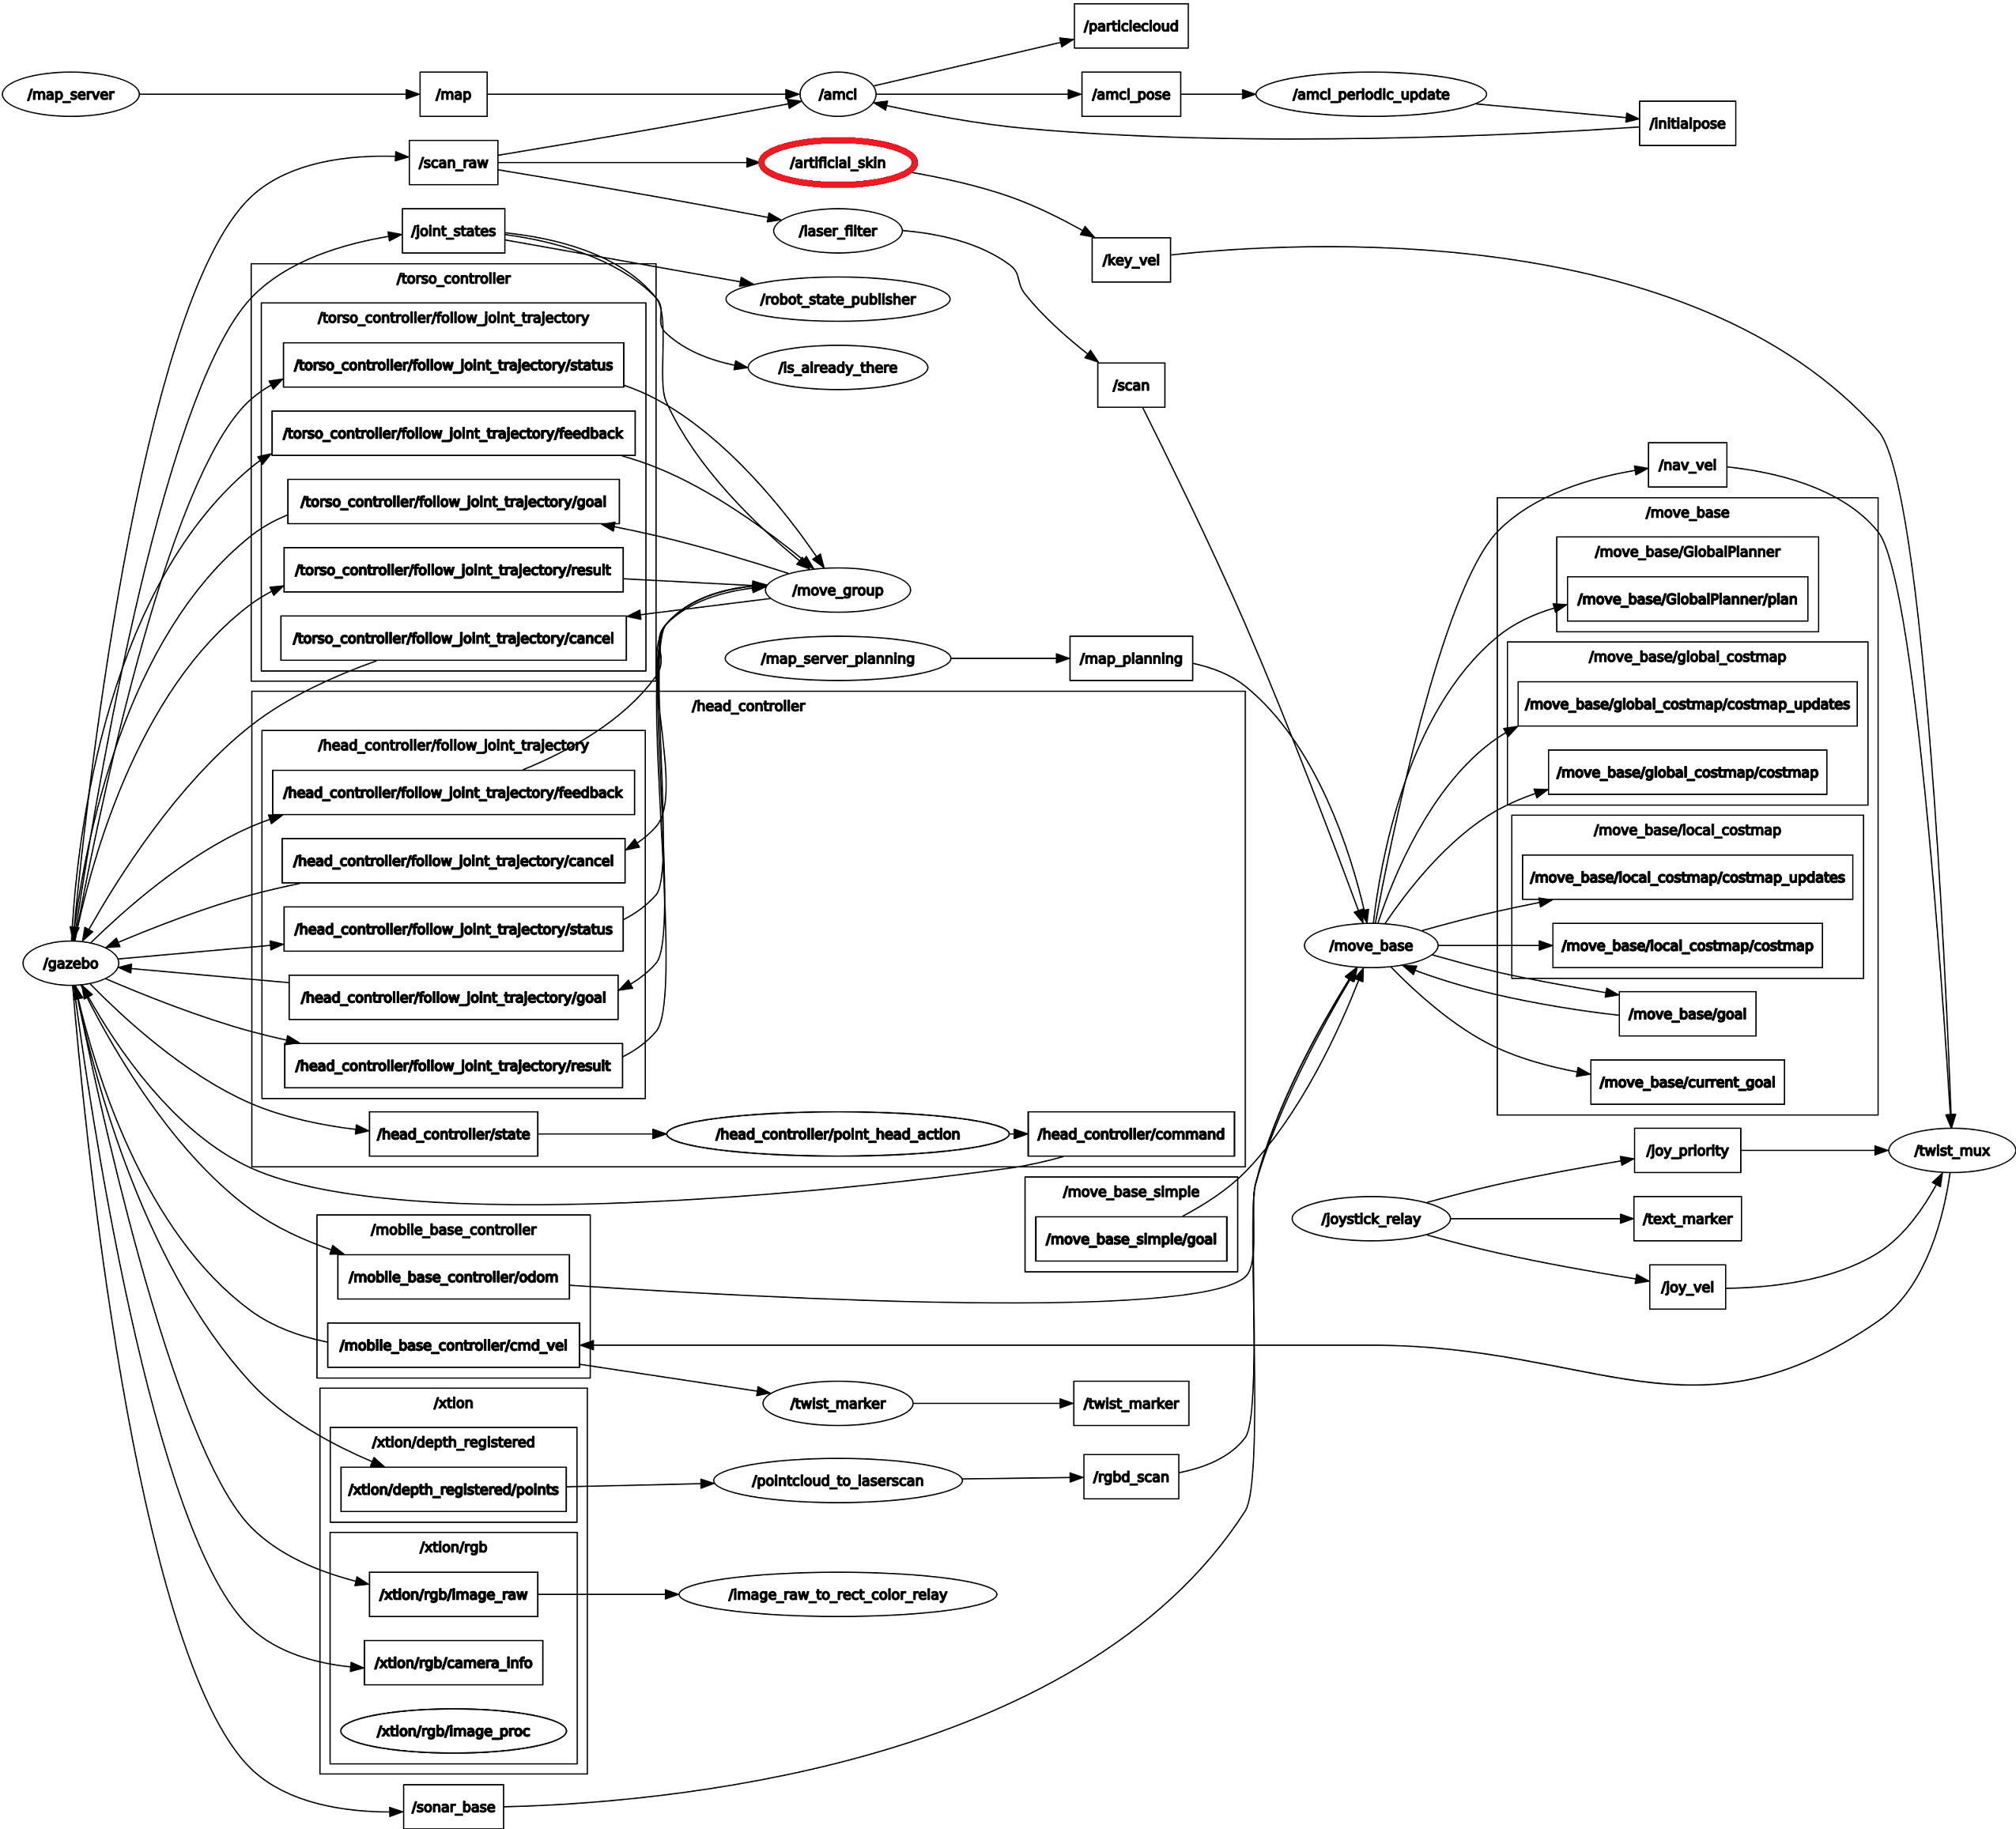
\includegraphics[width=1\linewidth]{img/ros_struktura.png}
    \caption{Struktura węzłowa robota Tiago wraz z dołączoną sztuczną skórą}
    \label{f_struktura_ros_integracja}
\end{figure}

% TODO zbieranie logów, czego xd

Integracja sztucznej skóry z robotem nastąpiła również pod względem mechanicznym. Została ona powieszona na robocie w górnej części, która jest trochę szersza niż tułów. Jako sposób mocowania zostały wybrane specjalnie zaprojektowane do tego celu i wydrukowane na drukarce 3D haczyki, które pozwalały na swobodne zakładanie i zdejmowanie modułu sztucznej skóry z robota. Sztuczna skóra została również podłączona do systemu za pomocą kabla USB łączącego ją z~notebookiem umieszczonym na robocie. Robot z~zamocowaną sztuczną skórą widoczny jest na rysunku \ref{f_czujnik_na_robocie}.

\begin{figure}
  \begin{subfigure}[t]{0.65\linewidth}
    \centering
    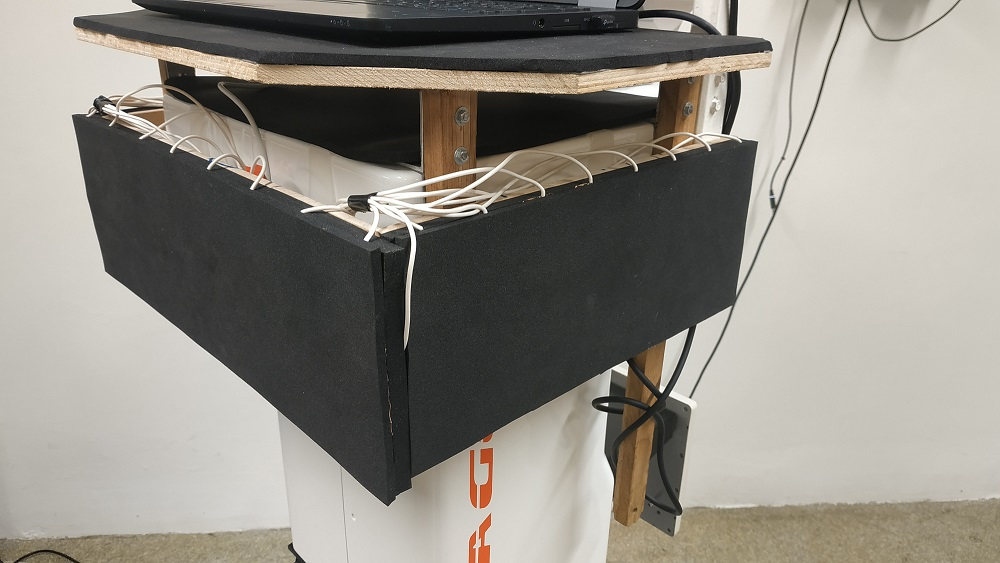
\includegraphics[width=0.9\linewidth]{img/czujnik_mocowanie_1.jpg} 
    \caption{Widok z bliska} 
    % \vspace{4ex}
  \end{subfigure}%% 
  \begin{subfigure}[t]{0.35\linewidth}
    \centering
    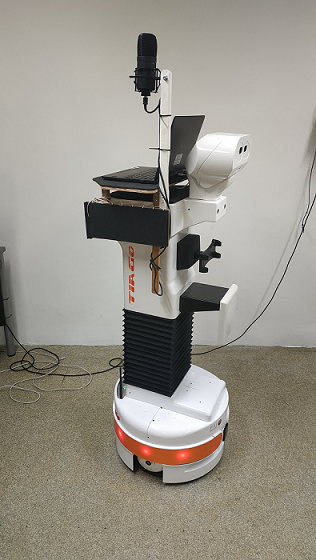
\includegraphics[width=0.9\linewidth]{img/czujnik_mocowanie_2.png}
    \caption{Widok całości robota} 
    % \vspace{4ex}
  \end{subfigure}
  \centering
  \caption{Zbudowany prototyp zamocowany na robocie}
  \label{f_czujnik_na_robocie}
\end{figure}

\subsection{Algorytm reakcji robota na wykryty nacisk}
\label{ss_integracja_algorytm}

Algorytm reakcji na nacisk jest jednym z kluczowych elementów w całym projekcie, zwieńcza on całe prowadzone badania. Ma on za zadanie interpretować przykładany nacisk i obliczać prędkość, z jaką poruszać się będzie robot. Podczas opracowywania algorytmu ściśle brano pod uwagę możliwości robota, a dokładniej ograniczenia, które nakłada różnicowy układ jezdny.

Opracowany algorytm wysyłający komendy sterowania uruchamiał się tylko w momencie, kiedy odczytane ze sterownika dane były niezerowe. Po otrzymaniu danych odczytana wartość siły jest przeliczana na lokalny mnożnik do wartości wystawianej na sterowaniu. Mnożnik ten jest uzyskiwany poprzez dzielenie otrzymanej siły pomiarów przez maksymalną wartość jaką sterownik może wysłać, czyli 10000 (a dokładniej 9999, ponieważ wartość siły jest zapisywana na 4 polach). % TODO w sumie to jest spierdolony kod napisałem
Dzięki temu prostemu zabiegowi odczytana wartość siły nie będzie się znajdowała w okolicach 1, czyli maksymalnej wartości jaka powinna być przesyłana do sterowania robota za pomocą tematu $/key\_vel$. Większe wysyłane wartości nie mają już żadnego wpływu na prędkość poruszania robota. Obliczony mnożnik jest podstawą do obliczenia siły ruchu, zarówno dla prędkości liniowej, jak i~obrotowej. Mnożnik ten został w trakcie testów doświadczalnie zmodyfikowany, ponieważ otrzymywane wartości okazały się zbyt niskie do płynnego sterowania robotem.

Dokładne ustalenie prędkości liniowej i kątowej zostaje obliczane na podstawie odczytanego kąta siły nacisku. Zastosowane podejście zostało pokazane na rysunku \ref{f_algorytm_kierunek_schemat}. Podstawą było odjeżdżanie robota w możliwy sposób od miejsca generującego nacisk.
Pokazane zachowanie zostało osiągnięte dzięki odpowiedniemu wykorzystaniu funkcji trygonometrycznych. W trakcie pierwszych testów okazało się, że wartości prędkości obrotowej robota są niewystarczające do satysfakcjonującego działania, dlatego zostały one dodatkowo zwiększone. Rozwiązanie to posiada pewne wady i istnieją momenty, w~których lepszym wyjściem jest zatrzymanie się, lecz jako propozycja działania prototypu zachowuje się dobrze.

\begin{figure}[!h]
    \centering 
    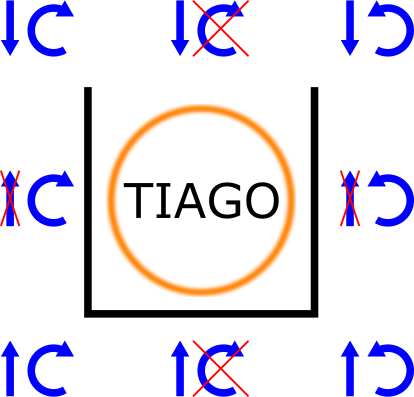
\includegraphics[width=0.5\linewidth]{img/kierunek_shcemat.png}
    \caption{Podstawowy schemat działania robota jako reakcja na wykryty nacisk}
    \label{f_algorytm_kierunek_schemat}
\end{figure}

Wadą zaproponowanego rozwiązania może być obracanie się robota przy otrzymaniu nacisku z boku, powodując jeszcze trochę zwiększenie tego nacisku. Jednocześnie jednak część tego nacisku zostanie przełożona na tylną część robota i robot pojedzie do~przodu, a~z~racji iż wciąż się obraca odjedzie od przeszkody. Jest to spowodowane przez kwadratową obudowę czujnika, która w~praktyce nie jest równo odległa od środka obrotu robota. Jedynym rozwiązaniem, które pozwala na wyeliminowanie tego problemu jest wykorzystanie czujnika opartego na okręgu. Wykonanie czujnika okrągłego dostarcza jednak dodatkowych problemów konstrukcyjnych, a prototyp kwadratowy jest wystarczający do~pierwszych testów.

Dodatkowo do kodu zostało wprowadzone zabezpieczenie przed uderzeniem w obiekty znajdujące się przed robotem podczas odjeżdżania od wywieranego nacisku. Byłoby to niefortunne, gdyby robot próbując uciec od jednego naciskającego obiektu uderzył w~inny. Aby mieć możliwość interpretowania odległości, węzeł sztucznej skóry odczytuje informacje ze skanera laserowego na temacie $/scan\_raw$. Dane te są przesyłane w opakowanej formie w wiadomości typu $LaserScan$ i zawierają pełną informację o~odczytanych odległościach do obiektów w zakresie działania skanera, czyli $\ang{220}$ ($\pm \ang{110}$). Tak duży zasięg wydawał się być niepotrzebny, dlatego do dalszych obliczeń brane były pod uwagę tylko obiekty znajdujące się bezpośrednio przed robotem i częściowo po jego bokach. Ustalono również zakres wykorzystywanych pomiarów na $\ang{180}$ ($\pm \ang{90}$). Interpretacja pomiarów była bardzo prosta - jeśli zostanie odczytany dystans poniżej $0,4m$ to należy zatrzymać robota. Jednocześnie z zatrzymaniem, robot wciąż ma możliwość obracania się, a nawet jego mnożnik do prędkości obracania się zostaje po raz kolejny zwiększony, aby szybciej znaleźć kierunek, w którym robot może odjechać.
